
\documentclass{article}
\usepackage{pgfplots}
\date{}

\title{\liningfont COP290 Assignment 2 \\ REPORT}
\author{\liningfont Anshik Sahu \quad 2021CS10577 \\ Aryan Dhaka \quad 2021CS50597 \\ Sanya Mittal \quad 2021CS10565}

\begin{document}

\maketitle
\thispagestyle{empty}
\pagestyle{empty}



\begin{abstract}
\noindent The assignment required us to give the cumulative count of words across N text files with the use of hashmaps. We had to then compare the performance, in terms of time elapsed to complete the operation on the same input files, across single threading and multiple threading, where multithreading was pre-implemented. 
\end{abstract}

\section{Introduction}

The following points are covered in the report:

\begin{itemize}
    \item Comparative analysis of single and multi-threading ie Part 2 and Part3 
    \item Implementation of locks to avoid race condition
    \item Data of file size Vs time (plots graphs and tables for the test)  
    \item Cause of difference in speeds of single and multi-threading
\end{itemize}

Part 1 of the assignment utilizes pointers to follow the process flow and track changes in function, while contexts are analogous to CPU registers and related functions like ucontext.

\section{Threading}
.
\subsection{Single vs Multi-threading}

\paragraph{Single threading} executes the process one at a time (concurrency) ie in the problem statement only one text file is handled at a time and other files are switched between one another but at any time only one file is being read. It uses the functions \texttt{mythread\char`_create}(makes the thread), \texttt{mythread\char`_join} (waits for the context to be executed after which it eliminates it from the stack), \texttt{mythread\char`_yield}(which executes the part of the context)

\paragraph{Multi threading} practices parallelism and executes multiple files under the same function,  in this case, all the input text files are read simultaneously. The functions for this are already provided.

\subsection{Locks and Race condition}
The introduction of locks in the single thread program rectified the race conditions, where two contexts were trying to work on the same word thus, the latter was not receiving the updated value by the first, rather both were simultaneously racing for the word. Thus when we were running two files with the same words then the count of the word was coming out to be incorrect because of race conditions. The introduction of locks made sure that only one context was incrementing the count at a time, thus the values were corrected. Thus the output varies. The output varies because  post introduction of locks because now if a context is incrementing a word count, the other waits until the first has completed working on that word. It continuously yields until the lock has been released by the previous context. And only then lets the new context have the lock.

\subsection{Comparative Testing}

The types of threading are compared on a variety of factors with the variables being the number of files, file size and cumulative file size 


\subsubsection{Single Varied size file}
\begin{tabular}{|c|c|c|}
\hline
 File Size(Mb) & Single-thread time(s) & Multi-thread time(s) \\
\hline
 0.43 & 0.08 & 0.10 \\
\hline
 1.3 & 0.16 & 0.16 \\
\hline
 6.5 & 0.66 & 0.46 \\
\hline
 11.4 & 1.13 & 0.75 \\
\hline
 34.5 & 3.34 & 2.16 \\
\hline
 45.8 & 4.45 & 2.83 \\
\hline
 69.1 & 6.61 & 4.28 \\
\hline
 80.5 & 7.75 & 5.01 \\
\hline
 91.8 & 8.82 & 5.89 \\
\hline
 126.3 & 12.11 & 7.79 \\
\hline
\end{tabular}

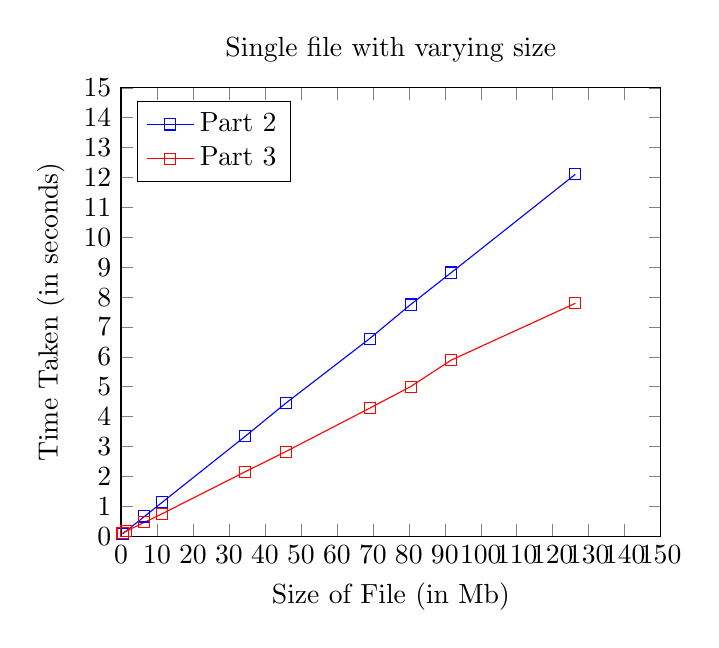
\begin{tikzpicture}
\begin{axis}[
    title={Single file with varying size},
    xlabel={Size of File (in Mb)},
    ylabel={Time Taken (in seconds)},
    xmin=0, xmax=150,
    ymin=0, ymax=15,
    xtick={0,10,20,30,40,50,60,70,80,90,100,110,120,130,140,150},
    ytick={0,1,2,3,4,5,6,7,8,9,10,11,12,13,14,15},
    legend pos=north west
]

\addplot[
    color=blue,
    mark=square,
    ]
    coordinates {
    (0.43,0.08)
    (1.3,0.16)
    (6.5,0.66)
    (11.4,1.13)
    (34.5,3.34)
    (45.8,4.45)
    (69.1,6.61)
    (80.5,7.75)
    (91.8,8.82)
    (126.3,12.11)

    };

\addplot[
    color=red,
    mark=square,
    ]
    coordinates {
    (0.43,0.098)
    (1.3,0.16)
    (6.5,0.465)
    (11.4,0.748)
    (34.5,2.156)
    (45.8,2.83)
    (69.1,4.282)
    (80.5,5.005)
    (91.8,5.893)
    (126.3,7.794)
    };
    \legend{Part 2, Part 3}

\end{axis}
\end{tikzpicture}

\paragraph{Observation:} Multi-threading is faster because more CPU resources are at the disposal 

\subsubsection{Same net file size with varying number of files}
\begin{tabular}{|c|c|c|}
\hline
 Number of Files & Single-thread time(s) & Multi-thread time(s) \\
\hline
 1 & 5.554 & 5.850 \\
\hline
 2 & 5.777& 3.408 \\
\hline
 4 & 2.937 & 2.033 \\
\hline

\end{tabular}


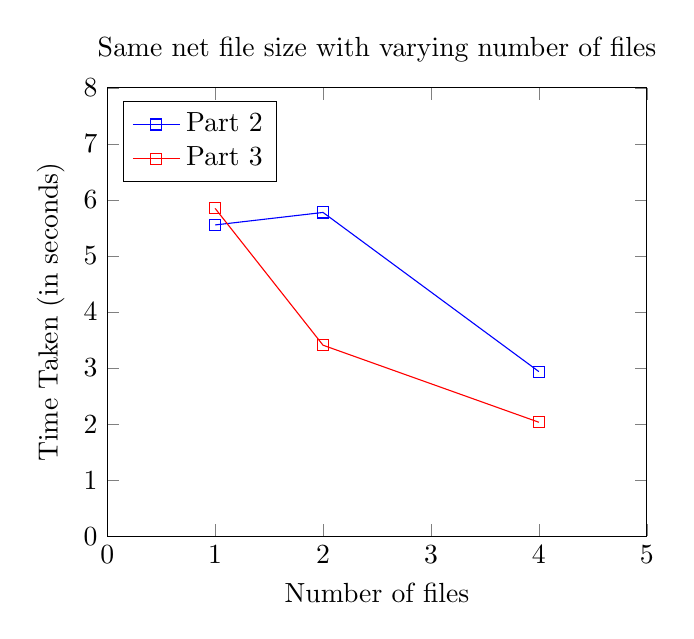
\begin{tikzpicture}
\begin{axis}[
    title={Same net file size with varying number of files},
    xlabel={Number of files},
    ylabel={Time Taken (in seconds)},
    xmin=0, xmax=5,
    ymin=0, ymax=8,
    xtick={0,1,2,3,4,5},
    ytick={0,1,2,3,4,5,6,7,8},
    legend pos=north west
]

\addplot[
    color=blue,
    mark=square,
    ]
    coordinates {
    (1,5.554)
    (2,5.777)
    (4,2.937)

    };

\addplot[
    color=red,
    mark=square,
    ]
    coordinates {
    (1,5.850)
    (2,3.408)
    (4,2.033)

    };
    \legend{Part 2, Part 3}
    
\end{axis}
\end{tikzpicture}

\paragraph{Observation :}Here one big file is step-wise split into 2 parts at each step. Multi-threading is faster for more files as they are executed simultaneously whilst the total characters across all files (total size) remains the same.

\subsubsection{Same single file size with varying number of files}
\begin{tabular}{|c|c|c|}
\hline
 Number of Files & Single-thread time(s) & Multi-thread time(s) \\
\hline
 1 & 1.305 & 1.370 \\
\hline
 2 & 2.602& 1.522 \\
\hline
 3 & 2.488 & 1.370 \\
\hline

\end{tabular}

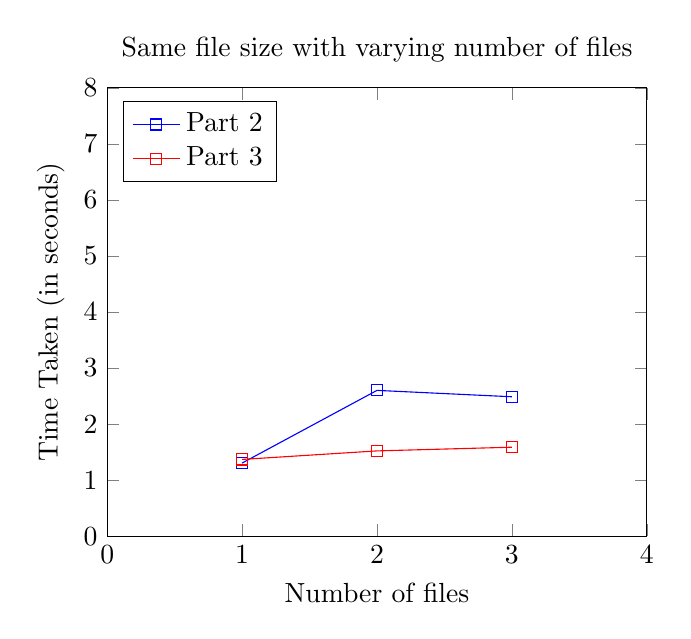
\begin{tikzpicture}
\begin{axis}[
    title={Same file size with varying number of files},
    xlabel={Number of files},
    ylabel={Time Taken (in seconds)},
    xmin=0, xmax=4,
    ymin=0, ymax=8,
    xtick={0,1,2,3,4},
    ytick={0,1,2,3,4,5,6,7,8},
    legend pos=north west
]

\addplot[
    color=blue,
    mark=square,
    ]
    coordinates {
    (1,1.305)
    (2,2.602)
    (3,2.488)

    };

\addplot[
    color=red,
    mark=square,
    ]
    coordinates {
    (1,1.370)
    (2,1.522)
    (3,1.588)

    };
    \legend{Part 2, Part 3}
    
\end{axis}
\end{tikzpicture}

\subsection{Why Multi-threading is faster?}

Multi-threading employs the use of more CPU power so the task that is, reading files is done faster due to the allocation of more resources. To simplify things, the procedure reads and processes more than one file at the same time, which ultimately speeds things up. This is the advantage of parallelism over concurrency, wherein more than one thing can be processed at the same time, and all the cores of the CPU are put to use parallel based on the number of threads. The creation of a new thread does take up some time, but this is more than made up for by the benefits described in the previous bullet point. This is also the reason why we observe relatively small time differences in small files, sometimes multi-threading even takes more time.

\section{Team Contribution}
\begin{center}
\begin{tabular}{|c|c|}
\hline
Name & Token \\
\hline
Anshik Sahu & 10 \\
\hline
Aryan Dhaka & 10 \\
\hline
Sanya Mittal & 10 \\
\hline
\end{tabular}
\end{center}

Anshik worked on hashmaps and threads. He implemented the hash table with keys and linked lists associated with each key, hashmap operations including get, put and thread operations including yield, create and join. He also worked on makefiles and race conditions, where the count values are incorrect when two contexts try to acquire the same key. 

Aryan worked on the theoretical aspects of threading and he developed the report on Latex, using tables and graphs. He deeply understood the differences in concurrency and parallelism and thus performed a comparative analysis in single and multi-threading along with data testing, and compared the graphs obtained via running the codes with the ideal scenario.

Sanya worked on the first part which was about storing and restoring contexts, on locks to rectify counts in single-threaded program, and in data testing for comparative analysis between single and multiple-threaded programs. She worked on the theoretical understanding of how and why locks rectify race condition errors. She also developed doxygen file for the code. 

We also worked collaboratively and helped each other with their aspects. We learned git and had a good experience with collaborative coding as well.

\end{document}
